%%
% The BIThesis Template for Bachelor Graduation Thesis
%
% 北京理工大学毕业设计(论文)第一章节 —— 使用 XeLaTeX 编译
%
% Copyright 2020-2022 BITNP
%
% This work may be distributed and/or modified under the
% conditions of the LaTeX Project Public License, either version 1.3
% of this license or (at your option) any later version.
% The latest version of this license is in
%   http://www.latex-project.org/lppl.txt
% and version 1.3 or later is part of all distributions of LaTeX
% version 2005/12/01 or later.
%
% This work has the LPPL maintenance status `maintained'.
%
% The Current Maintainer of this work is Feng Kaiyu.
%
% 第一章节

\chapter{绪论}

\section{研究背景}
三维场景地图的重建对三维计算机视觉、机器人学等领域有着重大意义,《“十四五”机器人产业发展规划》中指出,“机器人+”应用行动应该在汽车领域着力开发和推广,而自动驾驶的定位、场景理解离不开高逼真三维地图。三维场景重建的目的是从传感器拍摄的RGB图片、深度图、点云数据以及相机参数等信息中融合重建出三维场景地图。

特别的说,对于自动驾驶算法的迭代,建立一个具有真实感的仿真环境至关重要。通过在仿真环境中模拟具有挑战的道路环境,自动驾驶算法可以在较低成本下不断优化更新,从而提高其在实际路况中的表现。因此,三维场景重建技术在自动驾驶领域的应用也变得越来越重要。

在许多应用场景中,对于三维场景重建技术的要求越来越高,尤其是在场景外观和几何方面。在自动驾驶中,车辆需要通过三维场景地图来进行定位和路径规划,而场景的外观和几何结构直接影响车辆的感知和判断能力。如果场景的外观和几何结构与实际情况不符,那么车辆就很可能出现误判和错误的决策,导致安全隐患和交通事故的发生。因此,对于自动驾驶技术而言,对场景外观和几何的高精度要求更是不可或缺的。

传统显式的点云、栅格地图只能根据传感器分辨率在有限分辨率对场景进行描述,且对于存储的开销较大。近年来,基于神经网络的隐式地图得到了显著的发展,这类方法通过拟合一个隐式函数来对环境的关键物理量进行表征,从而对场景进行无限分辨率的表达。典型的隐式场有神经辐射场、神经有符号距离场等。

然而现有传统方法或单一隐式场方法不能同时建模较好的场景外观和精确的几何,从而限制了其在下游应用场景上的应用。如果使用混合的隐式表征(即混合隐式场),能够同时渲染逼真图片并且对于环境的几何形状有较为准确的表达,将会对下游重定位任务的执行、自动驾驶技术的提升等有巨大的帮助。

\begin{figure}[t]
    \centering
    \includegraphics[width=0.9\textwidth]{undergraduate-thesis/images/RGB-D.pdf}
    \caption{左图为神经辐射场渲染的RGB图片,右图为同样位姿下渲染的深度图。可以看到辐射场对于场景外观信息建模能力较强, 但对于场景几何的学习效果较差。}
    \label{fig:rgb-d}
\end{figure}

% 除此以外,由于神经辐射场中仅用“辐射”代替物理光照模型中光的全部传播规律,因此不能用于灵活地改变环境光照
现有混合隐式场方法尝试将距离函数映射为辐射场中用于体积积分的体密度\cite{wang_neus_2021, azinovic_neural_2022}。我们发现目前的混合隐式表征中存在诸多潜在的问题:
\begin{itemize}
    \item 目前方法中,通常使用一个函数映射将距离值转换为体密度,我们观察到现有转换方法中存在多视角误差,将会对几何表示学习产生较大影响。
    \item 同时优化多种隐式表达本质上是一个多目标优化问题,如果不对训练过程进行约束,将会显著影响每个隐式函数的优化结果。
    \item 现有方法存在训练慢、模型大、无法泛化到大场景等问题。
\end{itemize}

如图\ref{fig:rgb-d}可见,仅从RGB图片的单一传感器输入训练神经辐射场获得的场景深度图与真实值存在较大误差。使用深度损失函数等方式融入深度感知数据,然而由于这些方法的隐式场景表达本身存在多视角误差,深度信息的引入反而会影响优化问题的进行。

基于以上观察,我们提出“基于混合隐式场的多元传感融合场景表征”,希望在本课题中,解决或改善目前方法存在的不足。

\section{国内外研究现状}

神经辐射场(Neural Radiance Fields, NeRF)\cite{mildenhall_nerf_2020}最早被用于从已观测到的视角图片中学习场景信息,并渲染新视角下的图片,这类方法可以渲染高逼真的RGB图片。神经辐射场建立在一个简化的物理光照模型上:任意三维空间中的点均会向外散射不同颜色的光,从不同视角观察空间中的同一点的颜色可能不同,且每个点都会对其他方向传播过来的光线具有阻碍传播的作用。对三维点$P_i (x,y,z)$和观察角度$V(\theta,\phi)$,点$P_i$在角度V下观察到的颜色可以被一个五维连续隐式函数$f_{NeRF}:(x,y,z,\theta,\phi)\to (c_i,\sigma_i),c_i\in[0,255]^3,\sigma_i\in \mathbb{R}$ 建模,其中$c_i$为$P_i$散射出的RGB颜色值,而$\sigma_i$为该点的体密度。通过加权累积一条光线上所穿过点的辐射值,可以达到照片级的渲染,并且由于渲染过程的天然可微性,我们可以用渲染图片和观察到的图片之间的误差更新隐式函数$f_{NeRF}$。虽然神经辐射场可以精准地学习场景的视觉特征,然而仅从图片渲染误差中学习到的场景几何是缺乏约束的。因此,以神经辐射场为代表的方法在场景几何学习的深度估计等任务的精度要求上(如RMSE等指标)上的效果不足以支持“真实$\rightarrow$仿真$\rightarrow$真实”的任务要求,即将从视觉感知获得的几何表示应用于真实场景机器人实践应用(Real2Sim2Real)等更广泛的机器人应用。

相比神经辐射场主要通过图片中的特征学习场景的视觉信息,有符号距离场(Signed Distance Fields, SDF)可以用来表达更精确的场景几何信息。在有符号距离场 $f_{SDF}:(x,y,z)→d_i$中,任意空间点$P_i$被映射到其距离最近的表面的有符号距离$d_i\in \mathbb{R}$。通过从RGB图片中抽取多视角几何对应关系,或从深度图像中获取场景几何的直接观测结果,现有方法可以通过视觉感知输入重建较为准确的场景模型。然而这类方法通常无法得到逼真的RGB渲染图片。

\section{本课题主要工作及主要创新点}

近年来,混合隐式表达逐渐被研究者所关注,NeuS\cite{wang_neus_2021}方法首先提出了将辐射场和距离场相结合的范式,即建立距离到体密度的映射关系,然而该方法仅考虑了单视角下的无偏和遮挡,而没用考虑多视角的一致性,此外,该方法仅从RGB图片中学习场景表示,而不能利用深度图片的信息。NeuralRGB-D\cite{azinovic_neural_2022}方法在NeuS的基础上,使用了深度图来作为额外的场景感知输入。这些现有方法简单地将辐射场和距离场表达相结合,会使得整个优化任务的难度大大提升,从而显著地影响模型的整体性能。 因此,如何将不同的隐式函数有效地结合便成为当下隐式场研究的一个核心问题。为此,本课题首先考虑在场景的密度信息和梯度信息之间建立桥梁,保证混合隐式场在多视角下的空间一致性,实现距离场和辐射场的同时协同优化,以期解决隐式场的优化问题。除此以外,目前方法在表达大场景上存在严重的泛化问题,即训练速度极慢、模型大、效果差等。在本课题中,我们将考虑多元传感输入(包括RGB相机、激光雷达或深度相机等)下的三维场景,将不同模态下的传感数据进行融合,来优化混合隐式场表征。所得的混合隐式场应能被用于真实感的图像渲染、高保真深度预测和三维重建等应用场景。


\subsection{构建辐射场和距离场的理论桥梁}
\label{subsec:radiance2distance}
现有混合隐式表达方法通常将距离场中的数值$d$及其在空间上的梯度$\triangledown d$通过一个映射函数$g$转换为辐射场中的体密度$\sigma$。NeuS方法提出任何的转换函数$g$应满足的两个条件:
\begin{enumerate}
    \item \textbf{无偏性}:由$g\circ f_{SDF}$计算出的体密度应使一条光线在物体表面处的权重取得极大值;
    \item \textbf{遮挡感知}:当空间中两点$P_i$,$P_j$分别对应深度$t_i$,$t_j$满足$f_{SDF} (P_i )=f_{SDF} (P_j ),t_i<t_j$,则在渲染时须有权重$w_i>w_j$。
\end{enumerate}

然而这样的条件仅仅约束了同一条光线上权重分布的规律,而没有考虑空间中的对极几何约束,在本课题中,我们将分析该条件所产生的系统误差,并对不同隐式场之间转换的关系进行改进。

除此以外,在如NeuralRGB-D的现有的混合隐式场景表征方法中通常使用如式\ref{eq:depth-rendering}所示的数值积分计算渲染深度值,并用深度图对渲染深度对SDF分布进行约束。
\begin{equation}
    D = \frac 1 {\sum_{i=0}^{K-1}w_i}\sum_{i=0}^{K-1}w_i\cdot t_i
    \label{eq:depth-rendering}
\end{equation}

然而该方法使用深度图的数值作为有符号距离的估计值也存在天然的误差,从而进一步对场景几何表示学习带来困难。在本课题中,我们将使用视角相关的全方向距离场代替现有的有符号距离场表征来消除该误差。

\subsection{隐函数表示学习}
在最初的神经辐射场中,研究者使用多层感知机(Multi-layer Perceptrons, MLP)来建模隐函数$f_{NeRF}$,在MonoSDF\cite{yu_monosdf_2022}, InstantNGP\cite{muller_instant_2022}等后续工作中提出使用MLP来建模该函数关系存在训练/渲染时间过长、建模能力差和遗忘等问题,并提出使用三维空间网格代替感知机学习隐函数表征。但使用三维网格建模场景信息存在模型体积大,无法泛化到大场景的问题,因此后续工作\cite{chen_tensorf_2022, fridovich-keil_k-planes_2023, cao_hexplane_2023, reiser_merf_2023}提出使用张量分解\cite{kolda_tensor_2009}的思想将三维张量分解为多个二维矩阵,从而将场景模型的空间复杂度从$\mathcal O (L^3)$降为$\mathcal O (L^2)$。我们总结现有隐式场表示的方法如下作为可能的技术路线:
\begin{itemize}
    \item \textbf{多层感知机}:使用一个带残差的多层感知机分别学习混合隐式场表征。在查询时直接将空间点信息输入网络,直接预测隐函数值。如图\ref{fig:scene-representation} (a)所示。
    \item \textbf{空间体素网格}:使用一个空间体素网格存储空间中不同区域的隐式场真值,在推理时使用三线性插值计算任意给定三维空间中点的隐式函数值。如图\ref{fig:scene-representation} (b)所示。
    \item \textbf{多分辨率体素特征网格}:将三维空间按照不同分辨率分别建立空间体素网格,在网格中存储空间几何和外观的特征,并用三线性插值和一个浅层的解码器多层感知机推理隐函数值。
    \item \textbf{二维网格}:与空间体素网格相似,该类方法将隐式场表示为多个二维矩阵,在查询任意空间点的隐函数值时将该点投影到各个二维矩阵平面中,使用双线性插值得出投影点特征,将所有二维矩阵投影点的特征进行重新整合,得到最终查询点特征。如图\ref{fig:scene-representation} (c)所示。
    \item \textbf{混合表征}:同时多种相同或不同形式的隐式场表示方法。
\end{itemize}

\begin{figure}[t]
    \centering
    \includegraphics[width=\textwidth]{undergraduate-thesis/images/Scene Representations.pdf}
    \caption{场景表征示意图}
    \label{fig:scene-representation}
\end{figure}

\subsection{优化和约束混合隐式场}
\label{subsec:optimization}
在本课题中,我们将在原始神经辐射场的基于光度误差的隐式场优化方法的基础上,添加一系列约束条件来保证更好的网络优化。我们在本节中列出部分本课题中将使用的约束项:
\begin{itemize}
    \item \textbf{光度误差和深度误差}:通过在随机采样的渲染点上逐像素比对渲染RGB颜色/深度预测值和真实值的误差来优化隐函数。
    \item \textbf{距离场分布先验}:在全方向距离场中,一条光线上的理想距离值线性递减至0,本约束条件通过最小化采样光线和采样点上距离值和估计真值的误差来约束距离场分布。
    \item \textbf{距离场Eikonal先验}:有符号距离场中,空间中任意一点的隐函数梯度代表其朝向最近表面的法向向量。Eikonal先验\cite{wang_neus_2021}通过对梯度向量的模场进行限制来约束距离场数值大小。
\end{itemize}

\begin{figure}[t]
    \centering
    \includegraphics[width=\textwidth]{undergraduate-thesis/images/method.pdf}
    \caption{本课题中将采用的技术路线}
    \label{fig:method}
\end{figure}

\subsection{实验验证与评估}
\label{subsec:exp-and-evaluation}
本课题将在室内和室外大场景数据集上进行验证,并与基准算法进行对比实验,呈现本课题所提出的算法在图像渲染质量PSNR、深度预测误差RMSE以及重定位位姿误差等指标上的明显提升。在图\ref{fig:exp-scannet-rgb}、图\ref{fig:exp-real-lidar}中,我们展示了将被用于本课题数据集中的示例数据,包括不同模态的多元传感器数据。

\begin{figure}
    \centering
    \includegraphics[width=0.6\textwidth]{undergraduate-thesis/images/scannet-rgb.png}
    \caption{Scannet 数据集示例RGB图片}
    \label{fig:exp-scannet-rgb}
\end{figure}

\begin{figure}
    \centering
    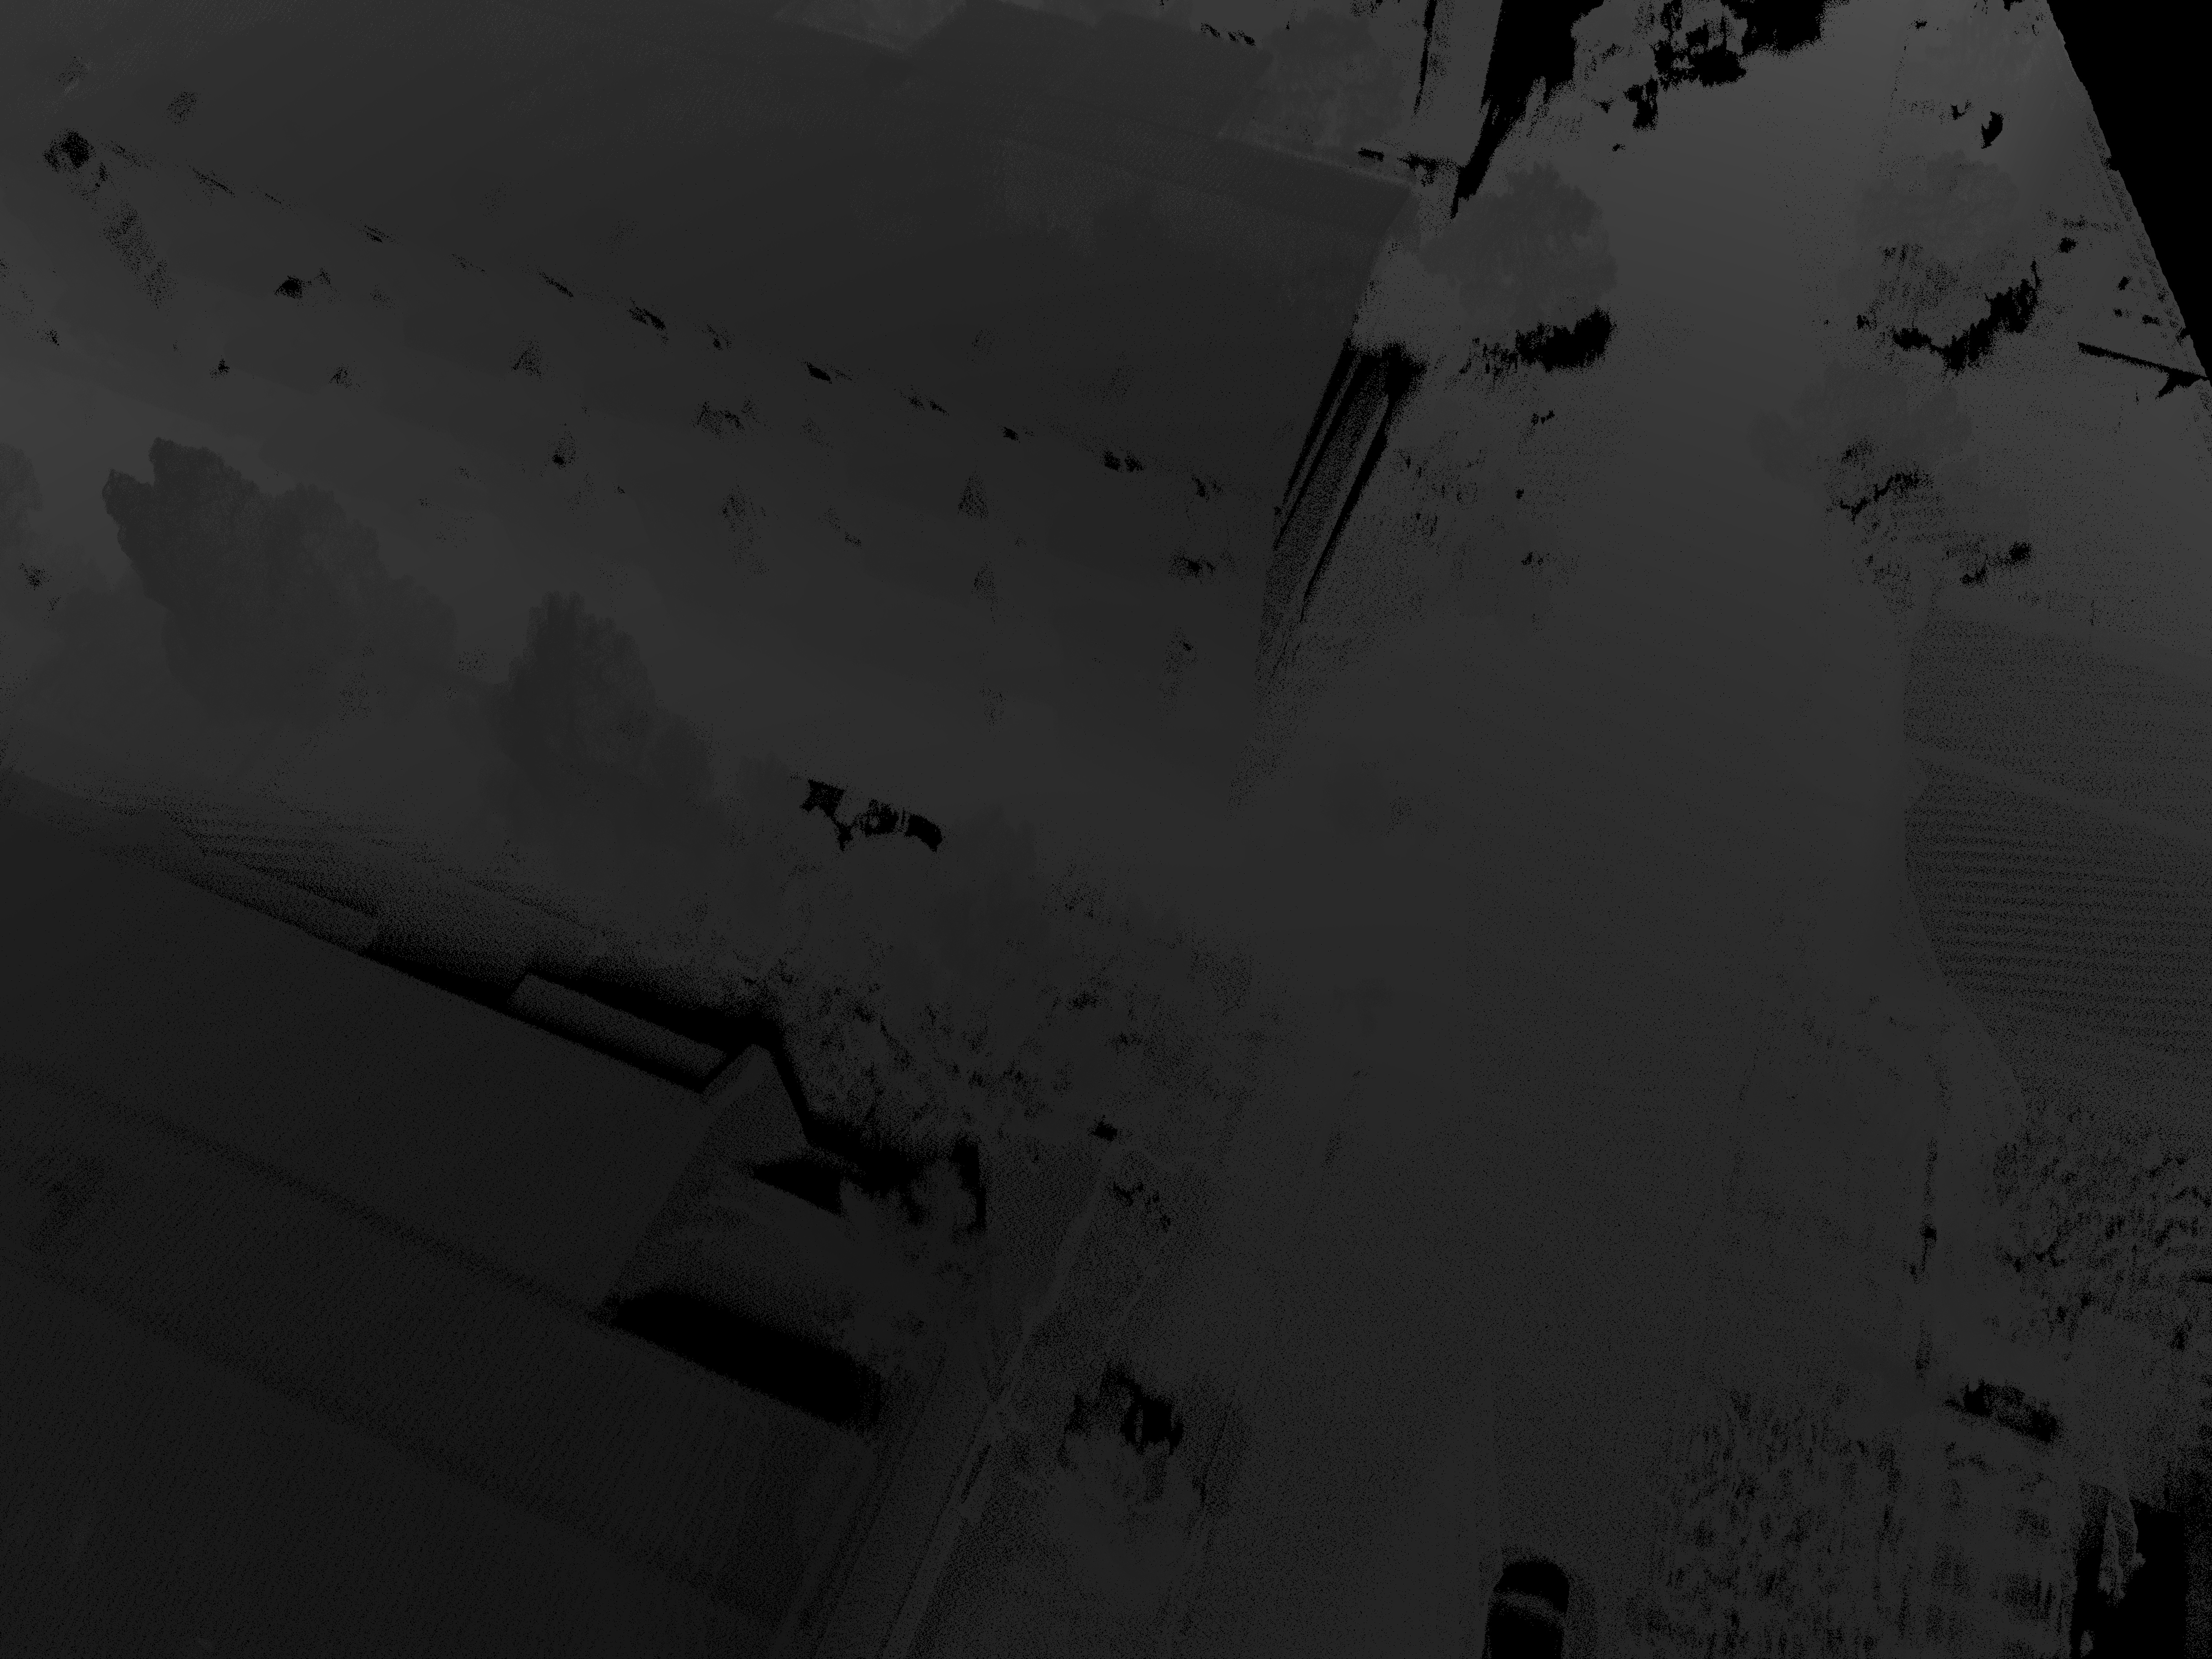
\includegraphics[width=0.6\textwidth]{undergraduate-thesis/images/pointcloud.png}
    \caption{真实数据集LiDAR点云数据(投影到二维平面后通过伪彩色映射进行可视化)}
    \label{fig:exp-real-lidar}
\end{figure}

\subsection{本文章节安排}

% 这里插入一个参考文献,仅作参考
% \subsection{三级题目}

% 正文……\cite{yuFeiJiZongTiDuoXueKeSheJiYouHuaDeXianZhuangYuFaZhanFangXiang2008}……\cite{Hajela2012Application}

% \textcolor{blue}{正文部分:宋体、小四;正文行距:22磅;间距段前段后均为0行。阅后删除此段。}

% \textcolor{blue}{图、表居中,图注标在图下方,表头标在表上方,宋体、五号、居中,1.25倍行距,间距段前段后均为0行,图表与上下文之间各空一行。阅后删除此段。}

% \textcolor{blue}{\underline{\underline{图-示例:(阅后删除此段)}}}


% \begin{figure}[htbp]
%   \centering
%   \includegraphics[]{images/bit_logo.png}
%   \caption{标题序号}\label{标题序号} % label 用来在文中索引
% \end{figure}

% \textcolor{blue}{\underline{\underline{表-示例:(阅后删除此段)}}}
% % 三线表
% \begin{table}[htbp]
%   \linespread{1.5}
%   \zihao{5}
%   \centering
%   \caption{统计表}\label{统计表}
%   \begin{tabular}{*{5}{>{\centering\arraybackslash}p{2cm}}} \toprule
%     项目    & 产量    & 销量    & 产值   & 比重    \\ \hline
%     手机    & 1000  & 10000 & 500  & 50\%  \\
%     计算机   & 5500  & 5000  & 220  & 22\%  \\
%     笔记本电脑 & 1100  & 1000  & 280  & 28\%  \\
%     合计    & 17600 & 16000 & 1000 & 100\% \\ \bottomrule
%     \end{tabular}
% \end{table}

% \textcolor{blue}{公式标注应于该公式所在行的最右侧。对于较长的公式只可在符号处(+、-、*、/、$\leqslant$ $\geqslant$ 等)转行。在文中引用公式时,在标号前加“式”,如式(1-2)。阅后删除此
% 段。}

% \textcolor{blue}{公式-示例:(阅后删除此段)}
% % 公式上下不要空行,置于同一个段落下即可,否则上下距离会出现高度不一致的问题
% \begin{equation}
%     LRI=1\ ∕\ \sqrt{1+{\left(\frac{{\mu }_{R}}{{\mu }_{s}}\right)}^{2}{\left(\frac{{\delta }_{R}}{{\delta }_{s}}\right)}^{2}}
% \end{equation}

% \subsubsection{生僻字}

% 一个可能无法正常显示的生僻字
% 一个可能无法正常显示的生僻字: 彧。下文注释中,介绍了如何通过自定义字体来显示生僻字。

% 定义一个提供了生僻字的字体,注意要确保你的系统存在该字体
% \setCJKfamilyfont{custom-font}{Noto Serif CJK SC}

% 使用自己定义的字体
% 使用提供了相应字型的字体:\CJKfamily{custom-font}{彧}。

